% Appendix E: The Rigorous Foundations of Integration (Riemann integral)

\begin{small}
\textit{Note: The concepts in this appendix go beyond the standard HSC Extension~2 Mathematics syllabus. They are provided as enrichment for students interested in university-level pure mathematics.}
\end{small}

\vspace{0.5em}

\subsubsection*{1. The Riemann Integral: A Formal Definition}

In the HSC syllabus, integration is often introduced intuitively as the ``area under a curve'' or the antiderivative. The \textbf{Riemann integral} (named after Bernhard Riemann) is a rigorous formulation of that area idea: we approximate the region by rectangles, then take a limit as the rectangles become arbitrarily thin.

Let $f$ be a bounded function on the closed interval $[a, b]$.

\begin{itemize}[leftmargin=*]
  \item \textbf{Partition.} We divide $[a, b]$ into $n$ subintervals using a partition $P = \{x_0, x_1, \dots, x_n\}$ with $a = x_0 < x_1 < \cdots < x_n = b$. The width of the $i$-th interval is $\Delta x_i = x_i - x_{i-1}$.
  \item \textbf{Norm.} The \textit{norm} (or mesh) of $P$, denoted $\|P\|$, is the largest subinterval width: $\|P\| = \max_i \Delta x_i$.
  \item \textbf{Sample points.} In each $[x_{i-1}, x_i]$ we choose any point $x_i^*$.
  \item \textbf{Riemann sum.} The corresponding Riemann sum is the total signed area of the approximating rectangles:
  \[
    S(P, f) = \sum_{i=1}^{n} f(x_i^*) \, \Delta x_i .
  \]
\end{itemize}

The function $f$ is \textbf{Riemann integrable} on $[a, b]$ if these sums stabilize to one number as the mesh goes to zero, no matter how the sample points are chosen: there exists $L \in \mathbb{R}$ such that
\[
  \int_a^b f(x) \, dx
  = \lim_{\|P\| \to 0} \sum_{i=1}^{n} f(x_i^*) \, \Delta x_i
  = L .
\]
Equivalently (and this is the usual $\varepsilon$--$\delta$ form of the same idea): for every $\varepsilon > 0$ there exists $\delta > 0$ such that whenever $\|P\| < \delta$ and $x_i^*$ are \emph{any} legal sample points,
  $|\,S(P,f) - L\,| < \varepsilon$.

\subsubsection*{2. A Worked Example: $f(x) = x$ on $[0, 1]$}

We show $\displaystyle \int_0^1 x \, dx = \tfrac{1}{2}$ from the limit of a Riemann sum.

\begin{enumerate}[leftmargin=*]
  \item \textbf{Regular partition.} Divide $[0, 1]$ into $n$ equal parts, so $\Delta x = 1/n$ and the grid points are $x_i = i/n$.
  \item \textbf{Sample points.} Take the right endpoint of each subinterval: $x_i^* = i/n$.
  \item \textbf{Riemann sum.}
  \[
    S_n = \sum_{i=1}^{n} f(x_i^*) \, \Delta x
        = \sum_{i=1}^{n} \frac{i}{n} \cdot \frac{1}{n}
        = \frac{1}{n^2} \sum_{i=1}^{n} i .
  \]
  \item \textbf{Limit.} Since $\sum_{i=1}^{n} i = n(n+1)/2$,
  \[
    S_n = \frac{1}{n^2} \cdot \frac{n(n+1)}{2}
        = \frac{1}{2} + \frac{1}{2n},
    \qquad\text{so}\qquad
    \lim_{n \to \infty} S_n = \frac{1}{2}.
  \]
  (Here $n \to \infty$ for this equal partition is one standard way to realize $\|P\| \to 0$.)
\end{enumerate}

\vspace{0.35cm}
\noindent\textbf{Diagram:} right-endpoint Riemann sum for $f(x)=x$ with $n=5$.

\begin{center}
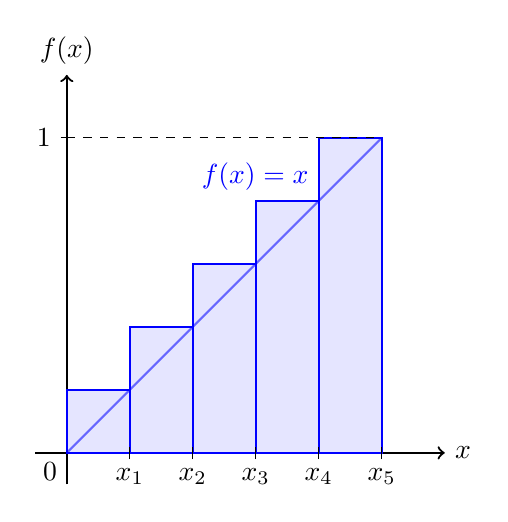
\begin{tikzpicture}[scale=4]
    \draw[->, thick] (-0.1, 0) -- (1.2, 0) node[right] {$x$};
    \draw[->, thick] (0, -0.1) -- (0, 1.2) node[above] {$f(x)$};
    \draw[thick, blue] (0,0) -- (1,1) node[pos=0.8, above left] {$f(x)=x$};
    \foreach \i in {1, 2, 3, 4, 5} {
        \pgfmathsetmacro{\x}{\i/5}
        \pgfmathsetmacro{\xprev}{(\i-1)/5}
        \draw[fill=blue!20, fill opacity=0.5, draw=blue, thick] (\xprev, 0) rectangle (\x, \x);
    }
    \foreach \x/\ticklab in {0.2/x_1, 0.4/x_2, 0.6/x_3, 0.8/x_4, 1.0/x_5} {
        \draw (\x, -0.02) -- (\x, 0.02);
        \node[below] at (\x, -0.02) {$\ticklab$};
    }
    \node[below left] at (0,0) {$0$};
    \draw[dashed] (0, 1) -- (1, 1);
    \draw (-0.02, 1) -- (0.02, 1);
    \node[left] at (-0.02, 1) {$1$};
\end{tikzpicture}
\end{center}

\subsubsection*{3. The Breaking Point: A Function That Is Not Riemann Integrable}

The Riemann integral behaves well for many functions you meet in school (e.g.\ bounded continuous functions on $[a,b]$), but it can fail for highly ``fractured'' behaviour. Define $f \colon [0,1] \to \mathbb{R}$ by
\[
  f(x) =
  \begin{cases}
    x & \text{if $x \in \mathbb{Q}$}, \\
    0 & \text{if $x \notin \mathbb{Q}$}.
  \end{cases}
\]
Every nonempty open interval in $[0,1]$ contains both rational and irrational numbers. So in each subinterval of any partition we can \emph{choose} sample points in two extreme ways:
\begin{itemize}[leftmargin=*]
  \item If every $x_i^*$ is rational, then $f(x_i^*) = x_i^*$, and for refined partitions the Riemann sums can be forced arbitrarily close to $\int_0^1 x\,dx = \frac{1}{2}$ (matching the integrable function $g(x)=x$).
  \item If every $x_i^*$ is irrational, then $f(x_i^*) = 0$, so every Riemann sum is exactly $0$.
\end{itemize}
Thus the limiting value of $S(P,f)$ as $\|P\| \to 0$ depends on how we choose sample points, so no single number $L$ satisfies the definition. Hence $f$ is \textbf{not Riemann integrable} on $[0,1]$.

\subsubsection*{4. University Preview: Where Integration Goes Next}

Beyond the HSC, analysis courses extend and refine integration.

\begin{itemize}[leftmargin=*]
  \item \textbf{Integrals in higher dimensions.} Volume under a surface $z = f(x,y)$ uses \textbf{double integrals}, e.g.\ $\displaystyle \iint_D f(x,y) \, dA$, built from small plane patches instead of intervals $\Delta x$.
  \item \textbf{Measure theory.} This develops a consistent notion of ``size'' (length, area, volume) for complicated sets. For instance, the rationals in $[0,1]$ have Lebesgue measure $0$, while the irrationals have measure $1$---a precise sense in which the rationals are negligible in length even though they are dense.
  \item \textbf{The Lebesgue integral.} Riemann integration slices the $x$-axis (horizontal partitions); Lebesgue's idea slices the \emph{range} of $f$ (vertical stacks). Informally: Riemann sums ``read'' the function left-to-right along the domain; Lebesgue integration groups points where $f$ takes similar values and measures how large those groups are. That theory integrates many functions Riemann cannot. For example, the rational/irrational function above satisfies $f(x)=0$ for almost every $x$ (the rationals have measure zero), so its Lebesgue integral on $[0,1]$ is $0$---a single definite value even though Riemann sums do not stabilize.
\end{itemize}
